\documentclass{beamer}

\usetheme{Antibes}
%\usetheme{split}
% this is a template for slides using beamer package
% adapted from slides written by Ramon Medrado
% first version: Ana Bazzan
\usecolortheme[RGB={120,0,0}]{structure}
\setbeamertemplate{blocks}[rounded][shadow=true]
\usepackage[latin1]{inputenc}
\usepackage{ragged2e}
\usepackage{graphicx}
\usepackage{caption}
\usepackage{booktabs}
\usepackage{subfig}
\usepackage{cite}

\begin{document}
\title{RGB-D Features Comparison in a Small Scale Localization Problem}
\section{Introduction}
\frame{
	\frametitle{Limited-Scope Localization with RGB-D Features}	
	\listoffigures
	\captionsetup{font=normalsize,labelfont={bf,sf}}
	\captionsetup[sub]{font=small,labelfont={bf,sf}}

	\begin{figure}[ht]
		\centering
		\label{figure:fig0}
		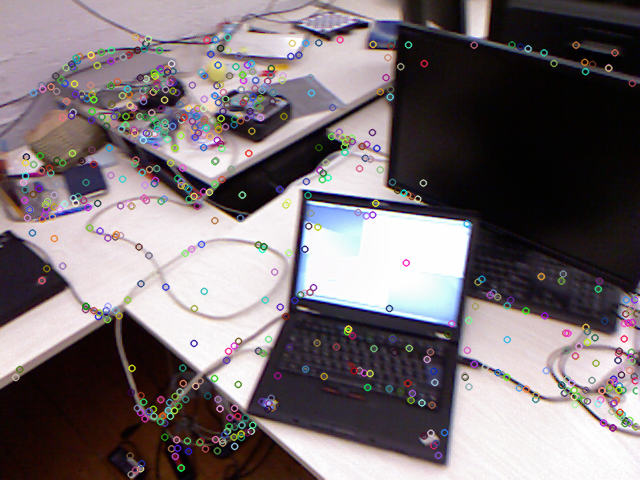
\includegraphics[scale=0.35, height=120pt, width=160pt]{siftkp}
		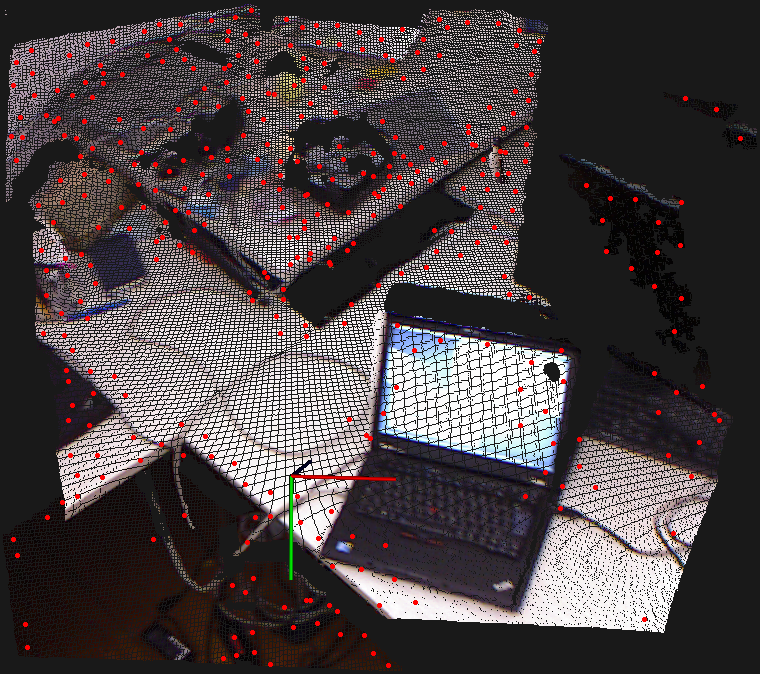
\includegraphics[scale=0.35, height=120pt, width=160pt]{narfdepthkp}
		\caption{SIFT RGB and NARF depth detected key points.}		
	\end{figure}
}

\section{Objective}
\frame{\frametitle{Objective}	
	\begin{itemize}
		\justifying
		\item Match image queries 		against an representative image database of an indoor environment;
		\item Set-up and use the BRAND\footnote{E. R. Nascimento, G. L. Oliveira, M. F. M. Campos, A. W. Vieira an W. R. Schwartz, "BRAND: A robust appearance and depth descriptor for RGB-D images," 2012 IEEE/RSJ International Conference on Intelligent Robots and Systems, Vilamoura, 2012, pp. 1720-1726.} RGB-D descriptor, comparing results against a well-known RGB descriptor;
		\item Start by applying RGB key point detectors following BRAND paper suggestions, and then investigate possible combinations with depth key point detectors.
	\end{itemize}
}

\section{Proposal}
\frame{\frametitle{Proposal}
	\begin{itemize}
		\justifying
		\item Database and query images selected from TUM \textit{fr1\_room} RGB-D indoor dataset:
		\begin{itemize}
			\justifying
			\item Whole environment was arbitrarily broke up in 16 representative images and loaded in a database;
			\item Four of the temporal sequence neighbors of each image were selected as queries, presenting slight perspective changes of the same scene elements;
		\end{itemize}
		\item SIFT descriptors as an alternative against BRAND;
		\item RGB Key points detected using OpenCV STAR, SIFT and combinations with NARF\footnote{B. Steder, R. B. Rusu, K. Konolige, and W. Burgard., "NARF: 3D Range Image Features for Object Recognition," In Workshop on Defining and Solving Realistic Perception Problems in Personal Robotics at the IEEE/RSJ Int. Conf. on Intelligent Robots and Systems (IROS). 2010.} and PCL SIFT for depth key points.
	\end{itemize}
}

\section{Development}
\frame{\frametitle{Development}
	\begin{columns}
		\begin{column}{0.5\textwidth}
			\begin{itemize}
				\justifying
				\item Conversion of RGB and depth images into a point cloud:
				\begin{itemize}
					\justifying
					\item Camera intrinsic parameters provided by TUM;
					\item TUM provided script outputs only PLY files with unorganized clouds;
					\item Alternative conversion was developed, receiving original dataset images and providing organized point cloud instances.
				\end{itemize}
				
			\end{itemize}
		\end{column}
		\begin{column}{0.5\textwidth}  %%<--- here
			\begin{center}
				\begin{figure}[ht]
					\centering
					\label{figure:fig1}
					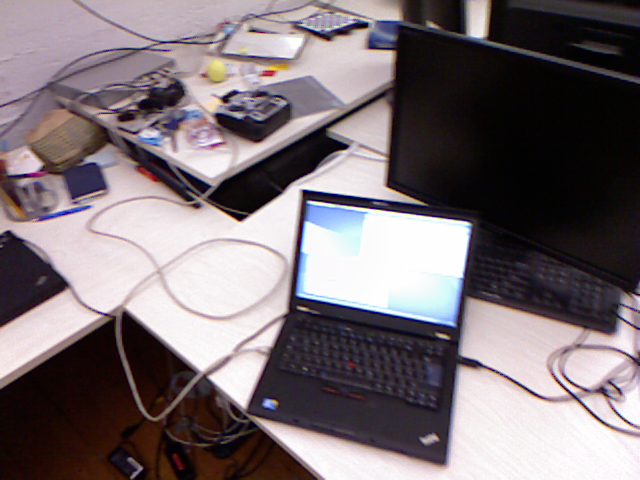
\includegraphics[scale=0.35, height=60pt, width=80pt]{rgb}
					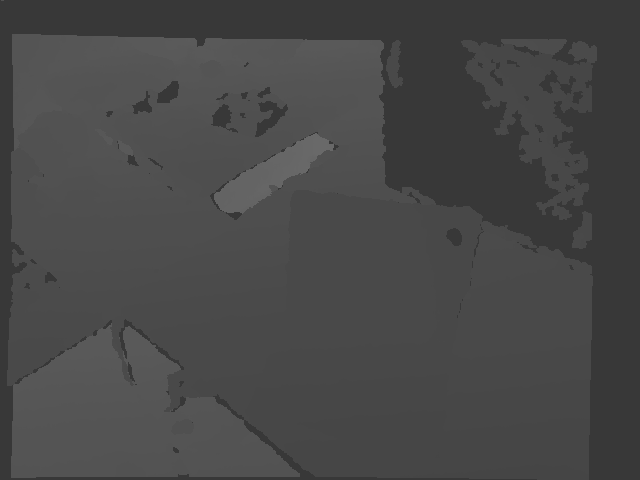
\includegraphics[scale=0.35, height=60pt, width=80pt]{depth}
					
					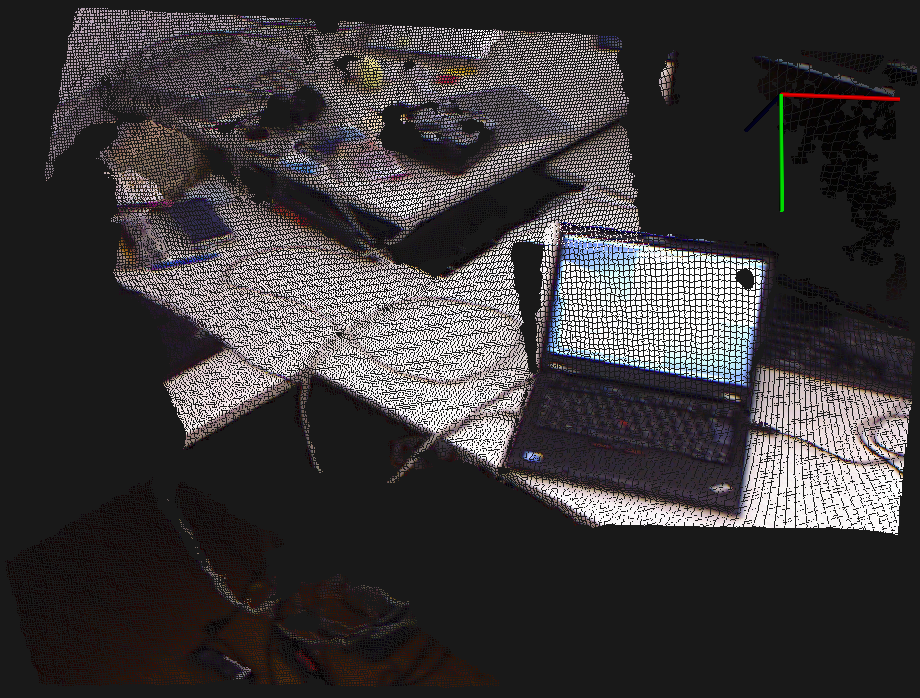
\includegraphics[scale=0.35, height=80pt, width=120pt]{cloud}
					\small
					\caption{RGB, depth and point cloud.}	
				\end{figure}
			\end{center}
		\end{column}
	\end{columns}
}

\frame{\frametitle{Development}
	\begin{itemize}
		\justifying
		\item Detection of SIFT and STAR RGB key points using OpenCV, with default parameters values:
		\begin{itemize}
			\item STAR is derived from CenSurE detector, both originally designed for real-time tasks as lightweight alternatives.
		\end{itemize}
		\begin{figure}[ht]
			\centering
			\label{figure:fig2}
			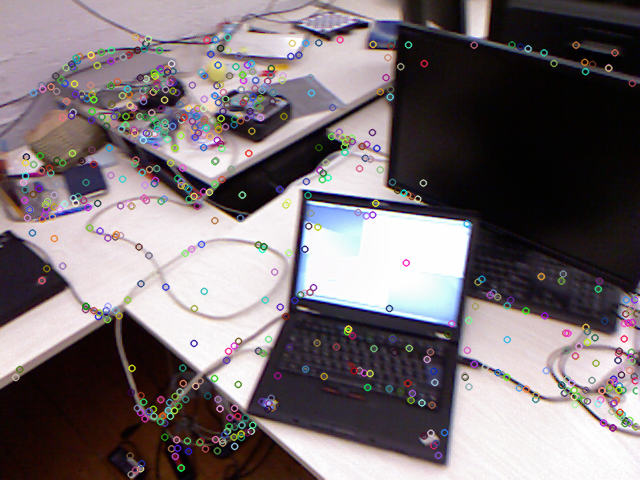
\includegraphics[scale=0.35, height=100pt, width=140pt]{siftkp}
			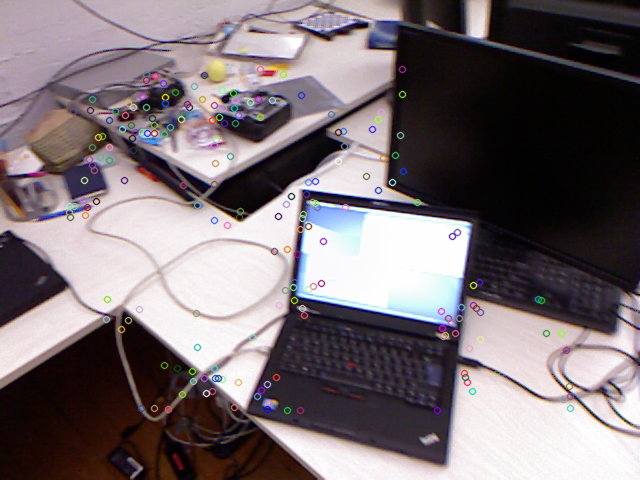
\includegraphics[scale=0.35, height=100pt, width=140pt]{starkp}
			\caption{SIFT and STAR detected key points.}		
		\end{figure}		
	\end{itemize}
}

\frame{\frametitle{Development}
	\begin{itemize}
		\justifying
		\item SIFT matching using L2 metric for descriptor distances, with outlier rejection via cross-checking, Lowe's distance ratio threshold at 75\%, and OpenCV RANSAC;
		\item BRAND matching using Hamming distance, with outlier rejection via cross-checking and OpenCV RANSAC;
		\item RANSAC first parameter increased from default value due to actual inliers rejection, while maintaining confidence parameter at default 99\%.
	\end{itemize}
}

\frame{\frametitle{Results - SIFT only}
	\begin{itemize}
		\justifying
		\item Queries for images 2, 4, 7, 11 and 15 have insufficient distinguishable matchings, results were very similar among different database images - particularly for image 2;
		\item Better candidate for a target 2 query with wrong result had 183 matchings (correct image had 151).
		\begin{figure}[ht]
			\centering
			\label{figure:fig3}
			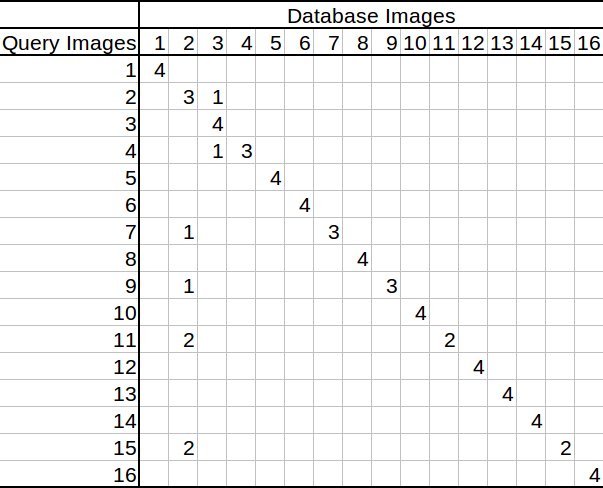
\includegraphics[scale=0.35, height=100pt, width=140pt]{siftnonesift}
			\caption{SIFT key points and descriptor matching results.}		
		\end{figure}		
	\end{itemize}
}

\frame{\frametitle{Results - STAR + BRAND}
	\begin{itemize}
		\justifying
		\item Queries for images 2 and 6 have insufficient distinguishable matchings in relation to their next image of the sequence;
		\item Queries for image 11 have very few inliers, results were similar among different database images.
		\begin{figure}[ht]
			\centering
			\label{figure:fig4}
			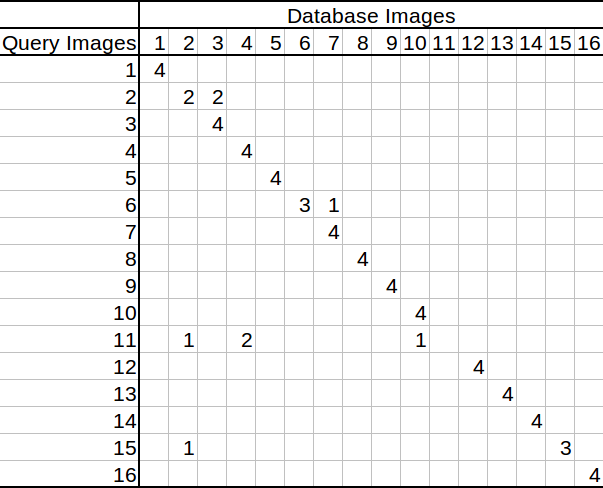
\includegraphics[scale=0.35, height=100pt, width=140pt]{starnonebrand}
			\caption{STAR key points + BRAND matching results.}		
		\end{figure}		
	\end{itemize}
}

\frame{\frametitle{Results - SIFT + BRAND}
	\begin{itemize}
		\justifying
		\item Queries for images 2, 11 have the lowest differences between better candidates and wrong alternatives (101-85 and 82-80 respectively).
		\begin{figure}[ht]
			\centering
			\label{figure:fig5}
			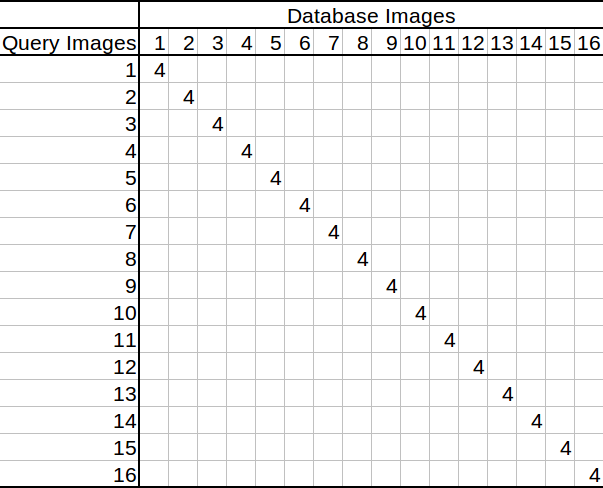
\includegraphics[scale=0.35, height=100pt, width=140pt]{siftnonebrand}
			\caption{SIFT key points + BRAND matching results.}		
		\end{figure}		
	\end{itemize}
}

\frame{\frametitle{Development}
	\begin{itemize}
		\justifying
		\item Detection of NARF depth key points using PCL, with default parameters values;
		\item NARF uses extracted borders from range images converted from point clouds, detecting key points on surface changes:			
		\begin{itemize}
			\item Detection behaves poorly near depth shadows and sensor limits.
		\end{itemize}
		\begin{figure}[ht]
			\centering
			\label{figure:fig6}
			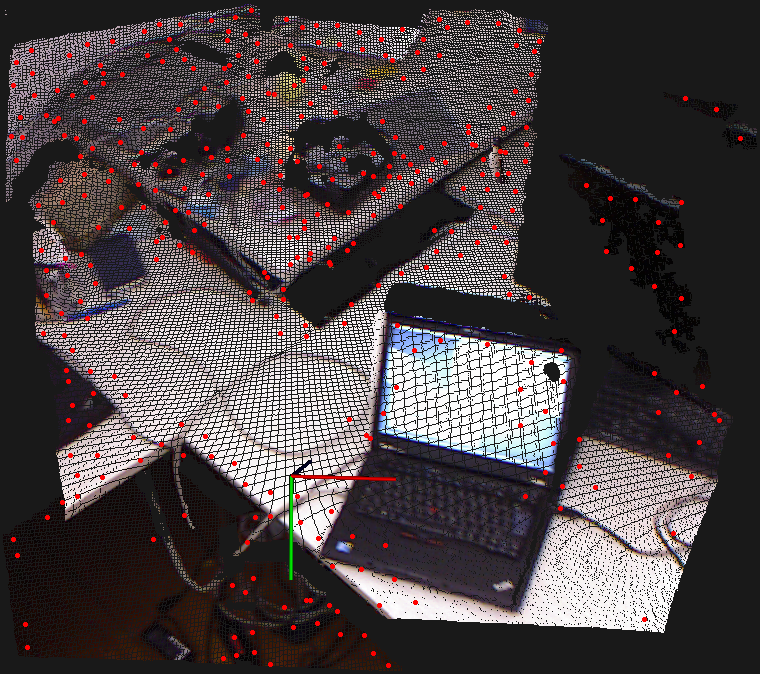
\includegraphics[scale=0.35, height=100pt, width=140pt]{narfdepthkp}
			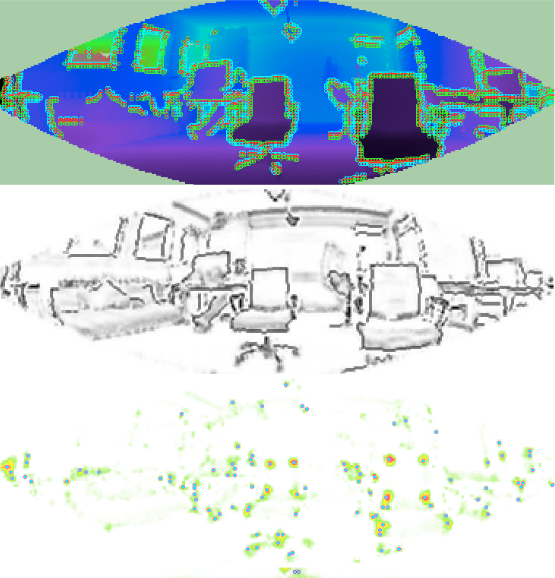
\includegraphics[scale=0.35, height=100pt, width=100pt]{narf}
			\caption{NARF key point detection.}		
		\end{figure}		
	\end{itemize}
}

\frame{\frametitle{Results - STAR + NARF + BRAND}
	\begin{itemize}
		\justifying
		\item BRAND matchings of detected NARF key points outnumbered STAR key points, alleviating its problems - particulary for image 11 queries;
		\item Unmatched descriptors and wrong matches have grown due to detection near depth shadows.
		\begin{figure}[ht]
			\centering
			\label{figure:fig7}
			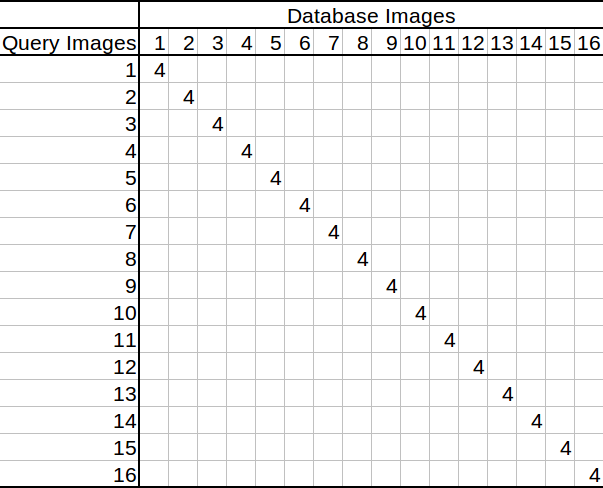
\includegraphics[scale=0.35, height=100pt, width=140pt]{starnarfbrand}
			\caption{STAR/NARF key points + BRAND matching results.}		
		\end{figure}		
	\end{itemize}
}

\frame{\frametitle{Development}
	\begin{itemize}
		\justifying
		\item Detection of SIFT depth key points using PCL, with default parameters values;
		\item Key points estimation was changed, using z gradient instead of intensity, following PCL documentation.
		\begin{figure}[ht]
			\centering
			\label{figure:fig8}
			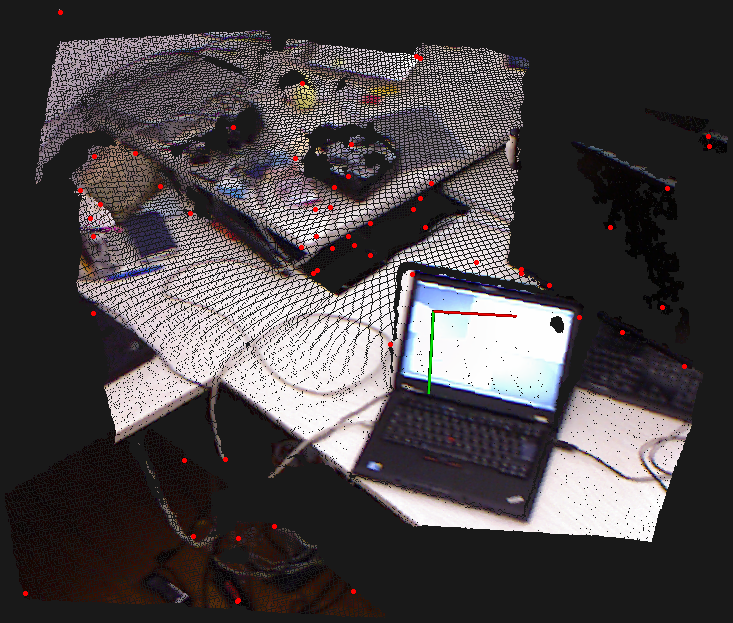
\includegraphics[scale=0.35, height=100pt, width=140pt]{siftdepthkp}
			\caption{PCL SIFT key point detection.}		
		\end{figure}		
	\end{itemize}
}

\frame{\frametitle{Results - SIFT RGB and depth + BRAND}
	\begin{itemize}
		\justifying
		\item Queries for images 2, 11 have the lowest differences between better candidates and wrong alternatives (123-93 and 97-95 respectively).
		\begin{figure}[ht]
			\centering
			\label{figure:fig9}
			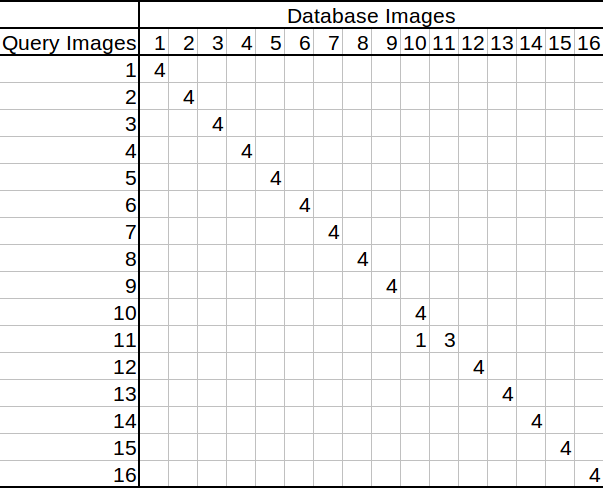
\includegraphics[scale=0.35, height=100pt, width=140pt]{siftsiftbrand}
			\caption{SIFT RGB and depth key points + BRAND matching results.}		
		\end{figure}		
	\end{itemize}
}

\frame{\frametitle{Conclusion}
	\begin{itemize}
		\justifying
		\item BRAND RGB-D descriptor matching improved with better key point detection (SIFT or STAR + NARF);
		\item SIFT RGB key points solved some issues of STAR use, but presented new problems;
		\item NARF depth key points helped alleviating some STAR issues, but behave poorly with depth shadows and sensor limits;
		\item SIFT depth key points failed to improve results, and have very slow detection process;
		\item Next steps:
		\begin{itemize}
			\item Investigate recent depth key point detectors and RGB-D descriptors (e.g. Serafin et al work, LOIND, RISAS) - some of them promise improvements upon NARF and BRAND.
		\end{itemize}
	\end{itemize}
}

\nocite{*}

\end{document}




